% Chapter 2: Propositional logic and claims (notes 2.1-2.5.2). Fragment: \input from the main file.
% Helper macros use the \log prefix so they can't clash with other chapters.
% \logCell{col}{row}{T or F}: one cell of a 2x2 assignment grid, shaded when the value is T
\newcommand{\logCell}[3]{%
  \if T#3\fill[gray!35] (#1*0.62,-#2*0.62) rectangle ++(0.62,-0.62);\fi
  \node[font=\scriptsize] at (#1*0.62+0.31,-#2*0.62-0.31) {#3};}
% \logGrid{xshift}{title}{TT}{TF}{FT}{FF}: satisfying assignments of a two-variable connective
\newcommand{\logGrid}[6]{%
  \begin{scope}[xshift=#1]
    \logCell{0}{0}{#3}\logCell{1}{0}{#4}\logCell{0}{1}{#5}\logCell{1}{1}{#6}
    \draw[step=0.62] (0,-1.24) grid (1.24,0);
    \node[font=\scriptsize] at (0.31,0.2) {$\mathrm{T}$};
    \node[font=\scriptsize] at (0.93,0.2) {$\mathrm{F}$};
    \node[font=\scriptsize] at (-0.22,-0.31) {$\mathrm{T}$};
    \node[font=\scriptsize] at (-0.22,-0.93) {$\mathrm{F}$};
    \node[font=\scriptsize] at (-0.3,0.25) {$P\backslash Q$};
    \node[font=\small] at (0.62,-1.62) {#2};
  \end{scope}}
\newcommand{\logT}{\mathrm{T}}
\newcommand{\logF}{\mathrm{F}}

\section{Propositional logic and claims}\label{logic:start}

The ideas in this chapter aren't hard. What costs points is \emph{evidence}, because the course is strict about it: a truth table with a skipped column, ``tautology'' with no table, ``not equivalent'' without naming the assignment that shows it. So along with the ideas, this chapter keeps saying exactly what you have to write down to back each one up.

% ------------------------------------------------------------------
\subsection{Propositions and expressions}

Compare ``$A\cap B$'' with ``$A\cap B=\varnothing$''. The first one names a thing (a set). The second one says something about that thing, and it's either true or false. That's the whole distinction.

\begin{notebox}
\textbf{Proposition.} A statement: something that asserts a fact and so is true or false (even if you don't know which yet, or it depends on a variable).\\
\textbf{Expression.} Something that names a value: a number, a set, a string. ``$x^2-3$'', ``$A\cup B$'', ``the set of odd primes''.
\end{notebox}

``$n^2+1$ is prime'' is a proposition, even though whether it's true depends on $n$. Questions (``Is 7 prime?''), commands (``Close the door.'') and bare noun phrases aren't propositions.

An \emph{atomic} proposition can't be split into smaller propositions. A \emph{compound} one is built from smaller ones with connectives. We use capital letters $P,Q,R$ for atomic propositions and lowercase $p,q$ for any formula.

\textbf{Where people slip.} Treating an expression as a statement. ``Assume $A\cap B$'' is nonsense, because you can't assume a set. You can assume $x\in A\cap B$.

% ------------------------------------------------------------------
\subsection{Connectives and truth tables}

There are six connectives. Each one is defined by its truth table: one row per combination of truth values for its parts.

\begin{center}
\begin{tabular}{cc|c|ccccc}
\toprule
$P$ & $Q$ & $\lnot P$ & $P\land Q$ & $P\lor Q$ & $P\oplus Q$ & $P\to Q$ & $P\leftrightarrow Q$\\
\midrule
T & T & F & T & T & F & T & T\\
T & F & F & F & T & T & F & F\\
F & T & T & F & T & T & T & F\\
F & F & T & F & F & F & T & T\\
\bottomrule
\end{tabular}
\end{center}

Names: $\land$ conjunction (``and''), $\lor$ inclusive disjunction (``or'', and both is fine), $\oplus$ exclusive disjunction (exactly one), $\lnot$ negation, $\to$ conditional (``if \dots\ then''), $\leftrightarrow$ biconditional (``if and only if'').

\begin{figure}[htb]
\centering
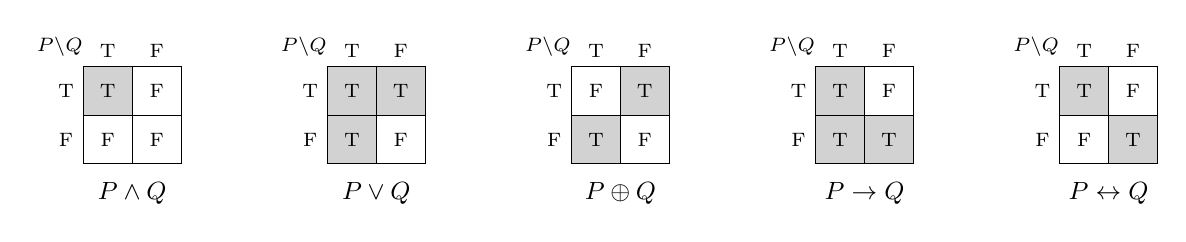
\begin{tikzpicture}
  \logGrid{0cm}{$P\land Q$}{T}{F}{F}{F}
  \logGrid{3.1cm}{$P\lor Q$}{T}{T}{T}{F}
  \logGrid{6.2cm}{$P\oplus Q$}{F}{T}{T}{F}
  \logGrid{9.3cm}{$P\to Q$}{T}{F}{T}{T}
  \logGrid{12.4cm}{$P\leftrightarrow Q$}{T}{F}{F}{T}
\end{tikzpicture}
\caption{The same tables as pictures. Each grid has one cell per truth assignment; shaded cells are the ones that satisfy the formula. $P\to Q$ has exactly one unshaded cell.}
\end{figure}

The one that trips people is $\to$. The way to remember it: a conditional is a promise, and the only way to break ``if $P$ then $Q$'' is to have $P$ happen and $Q$ not happen. That's the $(\logT,\logF)$ row. When $P$ is false, the promise was never tested, so the conditional counts as true. A few names you'll need: in $P\to Q$, $P$ is the \emph{premise} and $Q$ is the \emph{conclusion}.

\textbf{Where people slip.}
\begin{itemize}
  \item Making the bottom two rows of $P\to Q$ false. A false premise makes the whole conditional true.
  \item Using $\oplus$ for an ordinary ``or''. Inclusive is the default. Use $\oplus$ only for ``but not both'', ``exactly one of'', or very strong context.
  \item Writing $A\to B\to C$. Arrow isn't associative, so you must parenthesize. ($A\land B\land C$ is fine.)
  \item Mixing up the math symbols with code. In C, \texttt{\^{}} is exclusive or ($\oplus$), and there's no arrow at all.
\end{itemize}

% ------------------------------------------------------------------
\subsection{Translating English}

Translation goes in two steps. First, define atomic propositions, as small as you can, and keep the negation out of them (``$S$: the server is up'', not ``$S$: the server is down''). Then find the connective words and decide which chunk is a premise and which is a conclusion.

\begin{center}
\begin{tabularx}{\linewidth}{@{}Lc@{}}
\toprule
\textbf{English} & \textbf{Logic}\\
\midrule
$P$ and $Q$; $P$ but $Q$; $P$, yet $Q$; $P$, however $Q$ & $P\land Q$\\
$P$ or $Q$ (default); $P$ and/or $Q$; at least one of $P,Q$ & $P\lor Q$\\
exactly one of $P,Q$; $P$ or $Q$ but not both & $P\oplus Q$\\
neither $P$ nor $Q$ & $\lnot P\land\lnot Q$\\
$P$ unless $Q$ & $P\lor Q$\\
if $P$ then $Q$; $Q$ if $P$; $Q$ whenever $P$; $Q$ provided that $P$ & $P\to Q$\\
$P$ only if $Q$ & $P\to Q$\\
$P$ is sufficient for $Q$ & $P\to Q$\\
$P$ is necessary for $Q$ & $Q\to P$\\
$P$ if and only if $Q$; $P$ is necessary and sufficient for $Q$ & $P\leftrightarrow Q$\\
\bottomrule
\end{tabularx}
\end{center}

A few of these deserve a reason, so you can rebuild them under pressure:
\begin{itemize}
  \item \textbf{``But''} has the same truth table as ``and''. The contrast it adds is tone, not logic.
  \item \textbf{``Unless''} is an ``or'' word. ``We'll be there unless the car breaks down'' is false only if we aren't there \emph{and} the car didn't break down. That's the one $\logF$ row of $\lor$. (Context can push it to exclusive, but inclusive is the default.)
  \item \textbf{``If''} marks the premise wherever it appears in the sentence. So do ``whenever'', ``provided that'', ``in case'', ``given that''.
  \item \textbf{``Only if''} flips that: ``only'' plus a premise word marks the \emph{conclusion}. ``You can board only if you have a ticket'' means boarding $\to$ ticket. It does not promise that a ticket gets you on.
  \item \textbf{Sufficient} goes in the premise slot; \textbf{necessary} goes in the conclusion slot. Something necessary for $C$ is something $C$ can't happen without, so $C\to N$.
\end{itemize}

\textbf{Worked example.} Atoms: $S$ = ``the server is up'', $B$ = ``the backup ran'', $A$ = ``an alert fires''.
\begin{itemize}
  \item ``The server is up, but the backup didn't run.'' \quad $S\land\lnot B$
  \item ``An alert fires unless the backup ran.'' \quad $A\lor B$
  \item ``The backup runs only if the server is up.'' \quad $B\to S$
  \item ``The server being up is necessary for the backup to run.'' \quad $B\to S$ (the same claim as the last one)
  \item ``The backup running is sufficient for no alert.'' \quad $B\to\lnot A$
  \item ``Neither is the server up nor did the backup run.'' \quad $\lnot S\land\lnot B$
  \item ``An alert fires if and only if the server is down.'' \quad $A\leftrightarrow\lnot S$
\end{itemize}

\textbf{Where people slip.}
\begin{itemize}
  \item Translating ``$P$ only if $Q$'' as $Q\to P$. Read ``only if'' as ``then''.
  \item Putting the necessary condition in the premise.
  \item Reading an arrow as cause and effect. ``If there's smoke, there's fire'' is $\textit{smoke}\to\textit{fire}$, even though the fire causes the smoke. A conditional only says which combinations are allowed.
\end{itemize}

% ------------------------------------------------------------------
\subsection{Truth assignments and satisfaction}

A formula like $P\to Q$ isn't true or false on its own, any more than $x+y\leq5$ is. You need values for the variables first.

\begin{notebox}
\textbf{Truth assignment.} A choice of $\logT$ or $\logF$ for each atomic variable, e.g.\ $(P{=}\logT,Q{=}\logF)$.\\
\textbf{Satisfies.} An assignment satisfies a formula when the formula comes out $\logT$ under it.\\
\textbf{Satisfiable:} at least one assignment satisfies it.\quad
\textbf{Tautology:} every assignment satisfies it.\\
\textbf{Contradiction:} no assignment satisfies it.\quad
\textbf{Contingency:} at least one assignment satisfies it and at least one doesn't.
\end{notebox}

Say ``truth assignment'' and ``satisfying assignment'', never ``true assignment''. A truth table is just a tidy list of every assignment, one per row. With $n$ variables there are $2^n$ rows (same count as $|\mathcal{P}(A)|$ with $|A|=n$, because each variable is an independent in/out choice).

Every formula is exactly one of tautology, contingency, contradiction. Satisfiable means ``tautology or contingency''.

\begin{figure}[htb]
\centering
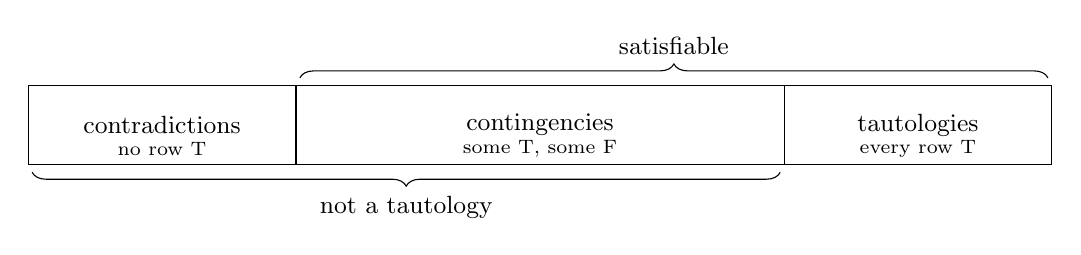
\begin{tikzpicture}[x=1cm,y=1cm]
  \draw (0,0) rectangle (3.4,1) node[midway,font=\small] {contradictions};
  \draw (3.4,0) rectangle (9.6,1) node[midway,font=\small] {contingencies};
  \draw (9.6,0) rectangle (13,1) node[midway,font=\small] {tautologies};
  \node[font=\scriptsize] at (1.7,0.2) {no row $\logT$};
  \node[font=\scriptsize] at (6.5,0.2) {some $\logT$, some $\logF$};
  \node[font=\scriptsize] at (11.3,0.2) {every row $\logT$};
  \draw[decorate,decoration={brace,amplitude=5pt}] (3.45,1.1) -- (12.95,1.1)
    node[midway,above=5pt,font=\small] {satisfiable};
  \draw[decorate,decoration={brace,amplitude=5pt,mirror}] (0.05,-0.1) -- (9.55,-0.1)
    node[midway,below=5pt,font=\small] {not a tautology};
\end{tikzpicture}
\caption{Every formula lands in exactly one box. ``Not a tautology'' covers two boxes, so it is not the same as ``contradiction''. Negating a formula swaps the two outer boxes and leaves a contingency a contingency.}
\end{figure}

\needspace{9\baselineskip}\textbf{Worked example.} Here are three formulas with every intermediate column written out.

\begin{center}
\begin{tabular}{cc|cc>{\bfseries}c|>{\bfseries}c|cc>{\bfseries}c}
\toprule
$P$ & $Q$ & $P\land Q$ & $\lnot(P\land Q)$ & $P\lor\lnot(P\land Q)$ & $(P\land Q)\land\lnot P$ & $\lnot P$ & $Q\land\lnot P$ & $P\to(Q\land\lnot P)$\\
\midrule
T & T & T & F & T & F & F & F & F\\
T & F & F & T & T & F & F & F & F\\
F & T & F & T & T & F & T & T & T\\
F & F & F & T & T & F & T & F & T\\
\bottomrule
\end{tabular}
\end{center}

$P\lor\lnot(P\land Q)$ is a tautology (all four rows $\logT$). $(P\land Q)\land\lnot P$ is a contradiction (all four $\logF$). $P\to(Q\land\lnot P)$ is a contingency: $(P{=}\logF,Q{=}\logT)$ satisfies it and $(P{=}\logT,Q{=}\logT)$ doesn't.

\textbf{What you have to show.} Learn this table. It tells you what a complete answer looks like for each kind of claim.

\begin{center}
\begin{tabularx}{\linewidth}{@{}lLL@{}}
\toprule
\textbf{Claim} & \textbf{To prove it} & \textbf{To disprove it}\\
\midrule
$p$ is satisfiable & one satisfying assignment (name it) & full table, no row $\logT$\\
$p$ is a tautology & full table, every row $\logT$ & one non-satisfying assignment, named explicitly\\
$p$ is a contradiction & full table, no row $\logT$ & one satisfying assignment\\
$p$ is a contingency & one satisfying \emph{and} one non-satisfying assignment & full table: all $\logT$ or all $\logF$\\
$p\equiv q$ & full table, the two columns identical & one assignment that satisfies one but not the other\\
\bottomrule
\end{tabularx}
\end{center}

The pattern: claims that say ``there is'' need one example; claims that say ``every'' or ``no'' need the whole table. Even when your table is on the page, write the witnessing assignment out in words.

\textbf{Where people slip.}
\begin{itemize}
  \item Skipping intermediate columns to save time. That's where evaluation mistakes hide, and a table with missing steps doesn't show your work.
  \item Calling a tautology a contingency (or the reverse) because one row was evaluated wrong. Recheck the $\to$ rows; that's where most errors are.
  \item Saying ``satisfiable'' and stopping. Give the assignment.
\end{itemize}

% ------------------------------------------------------------------
\subsection{Logical equivalence}

Two formulas can look nothing alike and still say the same thing.

\begin{notebox}
\textbf{Logical equivalence.} $p\equiv q$ when every assignment that satisfies one also satisfies the other. Equivalently, their final columns match row for row. (Another way to say it: $p\leftrightarrow q$ is a tautology.)
\end{notebox}

In this course you prove equivalence with a full truth table. Named rewriting laws (De Morgan's, distribution, and so on) are \emph{not} accepted as justification here. You may know them from elsewhere, and they're fine for guessing an answer, but the table is the proof.

\textbf{Worked example.} Is $\lnot(P\land Q)\equiv\lnot P\lor\lnot Q$?

\begin{center}
\begin{tabular}{cc|c>{\bfseries}c|cc>{\bfseries}c}
\toprule
$P$ & $Q$ & $P\land Q$ & $\lnot(P\land Q)$ & $\lnot P$ & $\lnot Q$ & $\lnot P\lor\lnot Q$\\
\midrule
T & T & T & F & F & F & F\\
T & F & F & T & F & T & T\\
F & T & F & T & T & F & T\\
F & F & F & T & T & T & T\\
\bottomrule
\end{tabular}
\end{center}

The two bold columns agree in every row, so yes, they're equivalent. Notice what the answer is made of: the table, plus the sentence saying the columns match.

When two formulas are \emph{not} equivalent, one row is enough, and you should name it. $P\to Q$ and $Q\to P$ differ at $(P{=}\logT,Q{=}\logF)$: that assignment satisfies $Q\to P$ but not $P\to Q$.

One more equivalence worth knowing because it describes how a conditional fails: $\lnot(P\to Q)\equiv P\land\lnot Q$. Check it with a four-row table yourself.

\textbf{Where people slip.}
\begin{itemize}
  \item Checking two or three rows and declaring the formulas equivalent. Matching on some rows proves nothing; every row has to match.
  \item Citing ``by De Morgan's law''. Here, that's an unsupported claim. Draw the table.
  \item Confusing $\equiv$ with $=$. $\equiv$ compares formulas across all assignments; $=$ is for sets and numbers.
\end{itemize}

% ------------------------------------------------------------------
\subsection{Converse, inverse, contrapositive}

Take a conditional $P\to Q$. Swap the parts, negate the parts, or do both, and you get three relatives:

\begin{center}
\begin{tabular}{lc}
\toprule
converse & $Q\to P$\\
inverse & $\lnot P\to\lnot Q$\\
contrapositive & $\lnot Q\to\lnot P$\\
\bottomrule
\end{tabular}
\qquad
\begin{tabular}{cc|>{\bfseries}cccc}
\toprule
$P$ & $Q$ & $P\to Q$ & $Q\to P$ & $\lnot P\to\lnot Q$ & $\lnot Q\to\lnot P$\\
\midrule
T & T & T & T & T & T\\
T & F & F & T & T & F\\
F & T & T & F & F & T\\
F & F & T & T & T & T\\
\bottomrule
\end{tabular}
\end{center}

Read the columns. The contrapositive matches the original in every row, so $P\to Q\equiv\lnot Q\to\lnot P$. The converse and the inverse each differ from the original (at $(\logT,\logF)$ and $(\logF,\logT)$), so neither is equivalent to it. They are equivalent to each other, though.

\begin{figure}[H]
\centering
\begin{tikzpicture}[x=5.2cm,y=2.1cm]
  \node[box] (o) at (0,1) {$P\to Q$\\[-2pt]\footnotesize original};
  \node[box] (c) at (1,1) {$Q\to P$\\[-2pt]\footnotesize converse};
  \node[box] (i) at (0,0) {$\lnot P\to\lnot Q$\\[-2pt]\footnotesize inverse};
  \node[box] (k) at (1,0) {$\lnot Q\to\lnot P$\\[-2pt]\footnotesize contrapositive};
  \draw[dashed] (o) -- node[lbl] {swap} (c);
  \draw[dashed] (o) -- node[lbl] {negate both} (i);
  \draw[dashed] (c) -- node[lbl] {negate both} (k);
  \draw[dashed] (i) -- node[lbl] {swap} (k);
  \draw[hl] (o) -- node[lbl,pos=0.3] {$\equiv$} (k);
  \draw[hl] (c) -- node[lbl,pos=0.3] {$\equiv$} (i);
\end{tikzpicture}
\caption{Thick diagonals join equivalent pairs (checked by the table above). Dashed sides are not equivalences.}
\end{figure}

\textbf{Worked example.} ``If a number is a multiple of 4, it's even.'' True for integers. Converse: ``if it's even, it's a multiple of 4'', false ($2$). Contrapositive: ``if it's odd, it's not a multiple of 4'', true, and it had to be, because it's equivalent to the original.

\textbf{Where people slip.} Assuming the converse because it ``feels'' like the same rule. People do this all the time outside class, too. If the course asks why two of these are or aren't equivalent, the answer is the table, not the vocabulary.

% ------------------------------------------------------------------
\subsection{Negation is not the opposite}

The negation of a statement is the statement that's true exactly when the original is false. That's often not the ``opposite'' that comes to mind.

\begin{itemize}
  \item ``He is tall'' negates to ``he is not tall'', not ``he is short''. Someone of medium height is neither tall nor short.
  \item ``$p$ is a tautology'' negates to ``$p$ is not a tautology'': some assignment fails to satisfy $p$. That's not the same as ``$p$ is a contradiction'' (see the figure in the satisfaction section).
  \item ``Every test case passed'' negates to ``at least one test case failed'', not ``every test case failed''.
  \item ``No integer squares to $-1$'' negates to ``some integer squares to $-1$''.
\end{itemize}

The general rule for claims about collections:

\begin{center}
\begin{tabular}{ll}
\toprule
\textbf{Claim} & \textbf{Negation}\\
\midrule
every $X$ is $Y$ & some $X$ is not $Y$\\
some $X$ is $Y$ & no $X$ is $Y$\\
no $X$ is $Y$ & some $X$ is $Y$\\
\bottomrule
\end{tabular}
\end{center}

Watch where you put the ``not''. The negation of ``some prime is even'' is ``no prime is even''. ``Some prime is not even'' is a true sentence, but it isn't the negation: it's true at the same time as the original ($2$ is an even prime, $3$ is an odd one).

\textbf{Where people slip.} Sticking ``not'' in the first grammatical spot that fits. Test your answer: exactly one of the original and your negation should be true, in every situation.

% ------------------------------------------------------------------
\subsection{Universal and existential claims}

Most claims you'll prove or disprove in this course are one of two kinds, and the kind tells you what kind of evidence you need.

\begin{notebox}
\textbf{Universal claim:} ``for every \dots'', ``all \dots'', ``no \dots'', ``if \dots\ then \dots''. Prove it by covering every case (one by one, or with a general argument). Disprove it with one counterexample.\\
\textbf{Existential claim:} ``there is \dots'', ``some \dots'', ``at least one \dots'', ``can'', ``possible''. Prove it with one example. Disprove it by showing every case fails.
\end{notebox}

Negating swaps the kind: the negation of a universal claim is existential, and the other way around. That's why one counterexample is enough to sink a universal claim.

The tricky part is that a lot of claims hide their quantifier inside a definition. Unpack it before you decide what evidence to give.

\begin{center}
\begin{tabularx}{\linewidth}{@{}lLc@{}}
\toprule
\textbf{Claim} & \textbf{What it says once you unpack it} & \textbf{Kind}\\
\midrule
$A\subseteq B$ & every member of $A$ is a member of $B$ & universal\\
$A=B$ & every member of either set is in the other & universal\\
$A\cap B=\varnothing$ & nothing is a member of both & universal\\
$p$ is a tautology & every assignment satisfies $p$ & universal\\
$p$ is not satisfiable & no assignment satisfies $p$ & universal\\
$n$ is prime & no $m$ with $1<m<n$ divides $n$ & universal\\
\midrule
$A\not\subseteq B$ & some member of $A$ isn't in $B$ & existential\\
$x\in\mathbb{Q}$ & there are integers $p,q$ ($q\neq0$) with $x=\frac pq$ & existential\\
$x\in\{n^2\mathrel{|} n\in\mathbb{Z}\}$ & some integer $n$ has $n^2=x$ & existential\\
$p$ is satisfiable & some assignment satisfies $p$ & existential\\
$p$ is a contingency & some assignment satisfies $p$ and some doesn't & existential\\
\bottomrule
\end{tabularx}
\end{center}

\textbf{Worked example.} ``$\{1,4,8\}\subseteq\{n^2\mathrel{|} n\in\mathbb{Z}\}$.'' Universal, so a single counterexample settles it: $8$ is in the left set and isn't a perfect square. False. Compare ``$9\in\{n^2\mathrel{|} n\in\mathbb{Z}\}$'': existential, so one witness settles it: $n=3$. True. (Membership in a set-builder set is existential, as in the sets chapter.)

\textbf{Where people slip.}
\begin{itemize}
  \item Proving a universal claim with one example. Examples prove existential claims only.
  \item Disproving an existential claim with one non-example. You need to rule out everything.
\end{itemize}

% ------------------------------------------------------------------
\subsection{Vacuous truth}

Here's a claim: ``Every member of $\{n\in\mathbb{Z}\mathrel{|} n^2<0\}$ is a prime number.'' True or false?

It's true. The set is empty, so there's nothing to check. To show it's false you'd need a counterexample, which would have to be a member of the set that isn't prime, and there are no members at all. A universal claim with no counterexample is true.

\begin{notebox}
\textbf{Vacuous truth.} A universal claim whose premise nothing can satisfy is true, whatever the conclusion says.
\end{notebox}

This is the same thing as the bottom two rows of the $\to$ table. When the premise is false, the conditional is true.

More examples:
\begin{itemize}
  \item $\varnothing\subseteq A$ for every set $A$. ``Every member of $\varnothing$ is in $A$'' has nothing to check.
  \item An empty dishwasher is ``all clean'' and also ``all dirty''. Both are vacuously true.
  \item $(P\land\lnot P)\to Q$ is a tautology. The premise is never satisfied, so no row can break it.
  \item The existential version flips: ``\emph{some} member of $\{n\in\mathbb{Z}\mathrel{|} n^2<0\}$ is prime'' is false, since there's no member to be the example.
\end{itemize}

\textbf{Where people slip.} Answering ``false'' or ``doesn't make sense'' because the conclusion sounds wrong, or because there's nothing to talk about. If the premise can't happen, the universal claim is true. Say so, and say why: ``vacuously true, since nothing satisfies the premise.''

% ------------------------------------------------------------------
\subsection{Practice}

None of these come from homework. For anything that needs a table, write every intermediate column.

\begin{enumerate}[label=\textbf{\arabic*.},leftmargin=1.8em,itemsep=0.35em]
  \item Proposition, expression, or neither?\\
  (a) ``$x+3$ is even'' \quad (b) ``the set of odd primes'' \quad (c) ``Close the door.''\\ (d) $\{1,2\}\cup\{3\}$ \quad (e) $\{1,2\}\subseteq\{3\}$ \quad (f) ``Is 7 prime?''
  \item Atoms: $R$ = ``it rains'', $G$ = ``the game is on'', $T$ = ``we have tickets'', $I$ = ``we get in''. Translate:\\
  (a) The game is on unless it rains. \quad (b) The game is on only if it isn't raining.\\
  (c) Having tickets is necessary for getting in. \quad (d) Rain is sufficient for the game to be off.\\
  (e) It's raining, but the game is on. \quad (f) We get in if and only if we have tickets and the game is on.\\
  (g) It's neither raining nor is the game on.
  \item (a) Does $(P{=}\logT,Q{=}\logF,R{=}\logT)$ satisfy $(P\to Q)\lor(Q\oplus R)$?\\
  (b) Does $(P{=}\logF,Q{=}\logF,R{=}\logF)$ satisfy $\lnot(P\lor R)\leftrightarrow Q$?
  \item Classify each as tautology, contradiction, or contingency, with the evidence the obligation table asks for:\\
  (a) $(P\to Q)\lor(Q\to P)$ \quad (b) $(P\leftrightarrow Q)\land(P\oplus Q)$ \quad (c) $(P\land\lnot Q)\to\lnot P$\\
  (d) $((P\to Q)\land\lnot Q)\to\lnot P$ \quad (e) $(P\lor Q)\to(P\lor R)$
  \item Equivalent or not? Prove your answer.\\
  (a) $\lnot(P\leftrightarrow Q)$ and $P\oplus Q$ \quad (b) $P\to(Q\to R)$ and $(P\land Q)\to R$\\
  (c) $(P\to R)\land(Q\to R)$ and $(P\land Q)\to R$ \quad (d) $\lnot(P\land Q)$ and $\lnot P\land\lnot Q$
  \item For integers: ``If $n$ is divisible by 6, then $n$ is even.'' Write the converse, inverse and contrapositive, and say which of the four statements are true.
  \item Negate each (a real negation, not an opposite):\\
  (a) Every bus today was late. \quad (b) Some password on the list is shorter than 8 characters.\\
  (c) The formula $p$ is a tautology. \quad (d) No square of an integer is negative.
  \item Say whether each claim is universal or existential (after unpacking), then whether it's true:\\
  (a) $\{4,9\}\subseteq\{n^2\mathrel{|} n\in\mathbb{Z}\}$ \quad (b) $12\in\{n^2-n\mathrel{|} n\in\mathbb{Z}\}$ \quad (c) $P\land\lnot P$ is not satisfiable\\
  (d) $\{1,2\}\neq\{2,1,1\}$ \quad (e) $P\to Q$ is a contingency
  \item True or false?\\
  (a) Every member of $\{n\in\mathbb{N}\mathrel{|} n<0\}$ is odd. \quad (b) Some member of $\{n\in\mathbb{N}\mathrel{|} n<0\}$ is odd.\\
  (c) Every truth assignment that satisfies $P\land\lnot P$ also satisfies $Q$.\\
  (d) Every subset $A$ of $\{7\}$ with $|A|=2$ is empty. \quad (e) ``If 3 is even, then 3 is prime.''
  \item (a) How many rows does a truth table with atoms $P,Q,R,S$ have?\\
  (b) A formula in $P$ and $Q$ has a final column of four $\logT$/$\logF$ entries. How many different final columns are possible? How many belong to tautologies, contradictions, contingencies?
  \item One friend says ``$P$ only if $Q$'' means ``if $Q$ then $P$''. Another says it means ``$Q$ is necessary for $P$''. Who's right? Back it up with a table.
\end{enumerate}

% ------------------------------------------------------------------
\subsection{Answers}

Every table and classification here was checked by brute force.

\begin{enumerate}[label=\textbf{\arabic*.},leftmargin=1.8em,itemsep=0.45em]
  \item (a) Proposition: it's true or false once $x$ has a value. (b) Expression: it names a set. (c) Neither: a command. (d) Expression: it names the set $\{1,2,3\}$. (e) Proposition (a false one, since $1\notin\{3\}$). (f) Neither: a question.
  \item (a) $G\lor R$. (b) $G\to\lnot R$. (c) $I\to T$ (necessary goes in the conclusion). (d) $R\to\lnot G$. (e) $R\land G$. (f) $I\leftrightarrow(T\land G)$. (g) $\lnot R\land\lnot G$.
  \item (a) $P\to Q$ is $\logT\to\logF=\logF$. $Q\oplus R$ is $\logF\oplus\logT=\logT$. So $\logF\lor\logT=\logT$. Yes, it satisfies the formula.
  (b) $P\lor R=\logF$, so $\lnot(P\lor R)=\logT$, and $\logT\leftrightarrow\logF=\logF$. No.
  \item Parts (a) and (b), with every intermediate column:

  \smallskip\begin{tabular}{cc|cc>{\bfseries}c|cc>{\bfseries}c}
  \toprule
  $P$ & $Q$ & $P\to Q$ & $Q\to P$ & (a) & $P\leftrightarrow Q$ & $P\oplus Q$ & (b)\\
  \midrule
  T & T & T & T & T & T & F & F\\
  T & F & F & T & T & F & T & F\\
  F & T & T & F & T & F & T & F\\
  F & F & T & T & T & T & F & F\\
  \bottomrule
  \end{tabular}\par\smallskip

  (a) \textbf{Tautology}: every row is $\logT$. (b) \textbf{Contradiction}: no row is $\logT$. The two parts can never agree, since $\oplus$ is $\logT$ exactly where $\leftrightarrow$ is $\logF$.

  Parts (c) and (d):

  \smallskip\begin{tabular}{cc|ccc>{\bfseries}c|cc>{\bfseries}c}
  \toprule
  $P$ & $Q$ & $\lnot P$ & $\lnot Q$ & $P\land\lnot Q$ & (c) & $P\to Q$ & $(P\to Q)\land\lnot Q$ & (d)\\
  \midrule
  T & T & F & F & F & T & T & F & T\\
  T & F & F & T & T & F & F & F & T\\
  F & T & T & F & F & T & T & F & T\\
  F & F & T & T & F & T & T & T & T\\
  \bottomrule
  \end{tabular}\par\smallskip

  (c) \textbf{Contingency}: $(P{=}\logF,Q{=}\logT)$ satisfies it and $(P{=}\logT,Q{=}\logF)$ doesn't. (d) \textbf{Tautology}: every row is $\logT$.

  (e) \textbf{Contingency}, and two assignments are all you need. $(P{=}\logF,Q{=}\logT,R{=}\logF)$: the premise $P\lor Q$ is $\logT$ and the conclusion $P\lor R$ is $\logF$, so it isn't satisfied. $(P{=}\logT,Q{=}\logT,R{=}\logT)$: both sides are $\logT$, so it is.
  \item (a) \textbf{Equivalent.} The full table:

  \smallskip\begin{tabular}{cc|c>{\bfseries}c>{\bfseries}c}
  \toprule
  $P$ & $Q$ & $P\leftrightarrow Q$ & $\lnot(P\leftrightarrow Q)$ & $P\oplus Q$\\
  \midrule
  T & T & T & F & F\\
  T & F & F & T & T\\
  F & T & F & T & T\\
  F & F & T & F & F\\
  \bottomrule
  \end{tabular}\par\smallskip

  The bold columns match in all four rows.

  (b) \textbf{Equivalent.} Eight rows this time:

  \smallskip\begin{tabular}{ccc|c>{\bfseries}c|c>{\bfseries}c}
  \toprule
  $P$ & $Q$ & $R$ & $Q\to R$ & $P\to(Q\to R)$ & $P\land Q$ & $(P\land Q)\to R$\\
  \midrule
  T & T & T & T & T & T & T\\
  T & T & F & F & F & T & F\\
  T & F & T & T & T & F & T\\
  T & F & F & T & T & F & T\\
  F & T & T & T & T & F & T\\
  F & T & F & F & T & F & T\\
  F & F & T & T & T & F & T\\
  F & F & F & T & T & F & T\\
  \bottomrule
  \end{tabular}\par\smallskip

  The bold columns match in all eight rows. Both formulas fail only when $P$ and $Q$ are true and $R$ is false.

  (c) \textbf{Not equivalent.} At $(P{=}\logT,Q{=}\logF,R{=}\logF)$: $P\to R$ is $\logF$, so the left side is $\logF$; $P\land Q$ is $\logF$, so the right side is $\logT$. That assignment satisfies the right formula but not the left. One row is enough.

  (d) \textbf{Not equivalent.} At $(P{=}\logT,Q{=}\logF)$: $\lnot(P\land Q)=\logT$ but $\lnot P\land\lnot Q=\logF$.
  \item Original: if $6\mid n$ then $n$ is even. True (a multiple of 6 is a multiple of 2).
  Converse: if $n$ is even then $6\mid n$. False, $n=2$.
  Inverse: if $6\nmid n$ then $n$ is odd. False, $n=2$ again.
  Contrapositive: if $n$ is odd then $6\nmid n$. True. It's equivalent to the original, so it had to be.
  \item (a) At least one bus today was not late. (b) Every password on the list has at least 8 characters. (c) Some truth assignment doesn't satisfy $p$. (Not ``$p$ is a contradiction''.) (d) Some integer has a negative square.
  \item (a) Universal (every member of the left is a square). True: $4=2^2$, $9=3^2$.
  (b) Existential (some integer $n$ gives $n^2-n=12$). True: $n=4$ works ($n=-3$ also does).
  (c) Universal (no assignment satisfies it). True: $P\land\lnot P$ is $\logF$ in both rows.
  (d) Existential (some member of one set isn't in the other). False: both sets are $\{1,2\}$.
  (e) Existential (one satisfying and one non-satisfying assignment). True: $(\logT,\logT)$ satisfies it, $(\logT,\logF)$ doesn't.
  \item (a) True, vacuously: no natural number is negative, so there's nothing to be a counterexample.
  (b) False: an existential claim needs a member to point at, and there isn't one.
  (c) True, vacuously: no assignment satisfies $P\land\lnot P$.
  (d) True, vacuously: $\{7\}$ has no two-member subsets.
  (e) True: the premise is false, so the conditional is true.
  \item (a) $2^4=16$.
  (b) Each of the four rows independently gets $\logT$ or $\logF$, so $2^4=16$ possible columns. Exactly one is all $\logT$ (tautologies), exactly one is all $\logF$ (contradictions), and the other $14$ are contingencies. Any two formulas with the same column are equivalent, so up to equivalence there are only 16 formulas in two variables.
  \item The second friend. ``$P$ only if $Q$'' is $P\to Q$, and ``$Q$ is necessary for $P$'' is also $P\to Q$, so they're literally the same formula. ``If $Q$ then $P$'' is $Q\to P$, the converse.

  \smallskip\begin{tabular}{cc|cc}
  \toprule
  $P$ & $Q$ & $P\to Q$ & $Q\to P$\\
  \midrule
  T & T & T & T\\
  T & F & F & T\\
  F & T & T & F\\
  F & F & T & T\\
  \bottomrule
  \end{tabular}\par\smallskip

  The columns differ at $(P{=}\logT,Q{=}\logF)$ (and at $(P{=}\logF,Q{=}\logT)$), so the first friend's version is not equivalent.
\end{enumerate}
